\chapter{Option Pricing, Heston Model}
\label{chapteroptionpricing}
\section{Introduction}

Now that we are done with Han Wong's paper, we proceed with the understanding of pricing, which is the second numerical topic I approached. We first define what it means to give a price to an asset, and then we price basic options like European call options. 

We go through a few technics, statistical as well as closed form. We also try to optimize those, in order to reduce the complexity of the methods; In particular we use the fft algorithm. All the methods can be generalized for more complex options types, but we will only focus on European call options. Those have the particularity to be easily computed and allows to focus on the technical issues of the methods.

Finally, we discuss quickly how well neural networks are able to approximate Black and Scholes.

\subsection{How to price options ?}

\begin{definition}[European Call Option]
$$C_T(K) :=  \Max (S_T - K, 0) =: (S_T - K)^+   $$
\end{definition}

One way to price financial instruments is to find a price where no arbitrage exists. This range of prices is called the arbitrage free prices. 

Equivalently thanks to the fundamental theorem of asset pricing, the price of any financial instrument, coined here $V_0$, is given by the expectation under a martingale / risk-free measure called $\mathbb Q$ of the discounted financial asset, or in other words for European call options:
$$V_0 = e^{-r T}  \mathbb E_{\mathbb Q} [ (S_T - K)^+ ] $$


\begin{theoreme}{Fundamental Theorem of asset pricing}
A model is said to be arbitrage-free i.e. there does not exist any admissible arbitrage strategy if and only if there exists an equivalent martingale measure $\mathbb Q$.
\end{theoreme}


There can be multiple different prices for the same option, thought in the case of a complete market, the price is unique. Under the Black and Scholes model, the market is complete and for that reason we find a unique price (B$\&$S model: appendix \ref{thrm:BSformula}). 



Also, one can equivalently price call or put option thanks to the put-call parity, which comes from the no arbitrage assumption: 


\begin{theoreme}{Put-Call parity}
$$C_t - P_t = S_t - \frac K {(1+r)^{T-t} }$$
\end{theoreme}











\section{Option Pricing Using Characteristic Functions}
\subsection{Theory}

\begin{definition}[Characteristic function]
The characteristic function is defined as the function associated to the random variable $X$ as:
\begin{align*}
  \phi_X \colon \mathbb R &\to \mathbb C \\
  \xi &\mapsto \mathbb E ( e^{i \xi X} ) 
\end{align*}

One can find some useful properties in \cite{num_methods}. One basic, though important, property that we are going to use is that $\phi_X$ is always hermitian, or formally: 

$$\phi_X( \xi ) = \conj{\phi_X} ( -\xi )$$


\end{definition} 




One classic example is the characteristic function for the dynamic of the asset under the Black-Scholes model:

\begin{equation}
\label{eq:charac_BS}
\phi_{X_t} (\xi) = \exp \left ( i \xi X_0 + ( r - \frac{ \sigma^2}{2}
) i \xi t - \frac{\sigma ^2 \xi ^2 t}{2} \right )
\end{equation}

More details in appendix \ref{anx:charac_BS}.

The advantage of pricing with a formula involving the characteristic function of a process over a formula with its density is that more functions have a useful characteristic function than a PDF. Many models do not allow for a closed-form representation of their density for their stock price process. On the other hand, the characteristic function is available to the class of affine models. Therefore, in many sophisticated models, it is easier to work with characteristics functions instead of using density functions.

Further on, we will need Gil-Pelaez Inversion Theorem (cf. \cite{gil_pelaez}), which states:

\begin{theoreme}{Gil-Pelaez Inversion Theorem}
If F is a one-dimensional distribution function and $\phi \colon \xi \to \int_{\mathbb R} e^{i \xi x} F(dx) $  its characteristic function, then we have the inverse formula for any
continuity point $x$ of $F$:

$$ F(x) = \frac 1 2 - \frac 1 { 2 \pi} \int_{\mathbb R} \frac{e^{- i x \xi } \phi ( \xi )  }  { i \xi }  d \xi $$

\end{theoreme}

Our aim is to write a computable expression for $C_T(k)$.


Remember that, writing $k = \ln(K)$, and $q_T$ is the pdf of $X_T$, the final log price of the asset, one can rewrite the pricing function as:

\begin{align}
C_T( k ) &=  e^{-r T}  \mathbb E_{\mathbb Q} [ (S_T - K)^+ ] \nonumber  \\
&= e^{-rT} \int_k^{\infty} e^x q_T(x) d(x) - K e^{-rT} \int_k^{\infty} q_T(x) dx \nonumber \\
&=: S_0 \Pi_1 - K e^{-r T} \Pi_2 
\label{eq:super_pricing}
\end{align}

(\ref{eq:super_pricing}) is, in the literature, usually referred as the "generalized" Black Scholes formula.

Also, remember that by hermitianity of $\phi_T$, one notices that:

$$ \mathfrak{R} ( \phi_T ( \xi) ) = \frac 1 2 \left ( \phi_T (\xi) + \phi_T (-\xi) \right ) \qquad  \text{ and } \qquad \mathfrak{I} ( \phi_T ( \xi) ) = \frac 1 {2i} \left ( \phi_T (\xi) - \phi_T (-\xi) \right ) $$

Gil-Pelaez inversion theorem applied to our pricing equation gives:

\begin{equation}
\label{eq:Pis}
\Pi_1 =  \frac 1 2 + \frac 1 {\pi} \int_0^{\infty} \mathfrak{R} \left ( \frac{ \phi_T ( \xi - i )  }  { i \xi \phi_T(-i) } e^{- i k \xi } \right ) d \xi  \qquad
\text{  and  }  \qquad
\Pi_2 =  \frac 1 2 + \frac {1} {\pi} \int_0^{\infty} \mathfrak{R} \left (  \frac{ \phi_T ( \xi )}    { i \xi } e^{- i k \xi } \right ) d \xi
\end{equation}

Using the function "real part" $ \mathfrak{R} $ allows to reduce truncation errors while computing an improper integral. 

Also, we used that $\phi_T(-i) = 1$. Remember

$$ \mathbb E ( e^{X_T} ) = \E ( S_T ) = S_0 $$ since we are working under the risk neutral measure for $S_t$.


Now, one is able to compute the price $C_T(k)$ by using (\ref{eq:Pis}) inside (\ref{eq:super_pricing}). This method presents two main advantages:

\begin{itemize}
\item \textbf{Generality:} For any process whose characteristic function is known, that method works.
\item \textbf{Semi-analytical solution:} by using integration routines, it is fairly easy to compute the pricing. Semi-analytical means the expression is in the form of the integral / Laplace or Fourier Transform of an analytical function. Numerical integration is described in the next section. 

\end{itemize}














\subsection{Integration}
\label{integration}

In order to compute $\Pi_1$ and $\Pi_2$, we need to integrate numerically a function. 

We are going to describe two different integration routines. For more details one can refer to the lecture notes of my second year lecture: in \cite{annalisa}, as well as in \cite{num_methods}. 

\begin{theoreme}{Trapezoidal Method}
$$\int_a^b f(x) dx = \frac 1 2 (f(a) + f(b))$$
It is first order exact and has the advantage of being extremely easy to use. For well-behaved functions (meaning whose second order derivates do not explode), the error is $ o (\frac 1 {n^2})$
\end{theoreme}


\begin{theoreme}{Simpson's Rule}
$$\int_a^b f(x) dx = \frac 1 6 (f(a) + 4 f(\frac{b-a}{2}) + f(b))$$
Simpson's method is much more precise as this method is third order exact and its error is $o (\frac 1 {n^4})$.
\end{theoreme}

\begin{remarque}
While trapeze's error is related to the second derivative of the function, Simpson's error is related to the fourth order derivative; more details in \cite{annalisa}. 
\end{remarque}


\begin{figure}
\centering
\includegraphics[width = 0.5 \textwidth]{../addition_part/images/integration_fft/numerical_integration.jpg}
\caption{Graphical explanation of the two quadratures method, images from \cite{annalisa}. Left: trapezoidal quadrature, right: Simpson's method.}
\end{figure}









\subsection{Overview of the different methods}
In order to compute the integrals, one needs the evaluation of the integrand at the desired points. Under the Heston model, we are lucky to have a closed form formula. However, as a first step, let me present a (failing) method to estimate the characteristic method. Another better and faster option for estimating the price is to directly compute the empirical price. The latter method is presented in section \ref{empirical_price}.

\subsection{Estimation of the characteristic function }


Following the definition of the characteristic function, one can estimate $\phi_X$ by estimating the PDF of the asset at maturity. Indeed, remember that:

$$\phi_{X_T} (\xi) = \mathbb E [ e^{i \xi X_T } ] = \int_{\mathbb R} e^{i \xi x } f_{X_T}(x) dx $$

I thought about two estimation methods:

\begin{itemize}
\item discrete: one approaches the PDF by the histogram. A classical result from statistics proves that the histogram of a random variable converges in probability to its PDF under certain conditions (cf. \cite{panaretos}).
\item continuous: using KDE, one can smoothen up the histogram and get a continuous PDF that should be close to the true PDF for the same reasons.
\end{itemize}

Figure \ref{fig:histogram_S} shows all the simulated final realisations of the process. 





\begin{figure}
\centering
\includegraphics[width = 0.8 \textwidth]{../addition_part/images/integration_fft/histogram_real.png}
\caption{Histogram of the final realisations of the simulated process.}
\label{fig:histogram_S}
\end{figure}

Based on that histogram, KDE algorithm has been applied leading to the figure \ref{fig:histogram_S_KDE}.




\begin{figure}
\centering
\includegraphics[width = 0.7 \textwidth]{../addition_part/images/integration_fft/histogram_real_kde.png}
\caption{KDE applied upon the histogram fig. \ref{fig:histogram_S}.}
\label{fig:histogram_S_KDE}
\end{figure}











\subsection{Results for continuous estimation} 

\begin{table}
\begin{center}
\begin{tabular}{   m{4.5 cm} | m{4.5 cm}   } 
\hline
Parameter & Value \\ 
\hline
\hline
$\sigma$ & 0.1  \\
\hline
$V_0$ &  0.1 \\
\hline
$X_0$ &  1 \\
\hline
$r$ & 0.0 \\
\hline
$\rho$ & -0.56 \\
\hline
$\theta$  & 0.07  \\
\hline
$\kappa$ & 1 \\
\hline
$\phi$ & 1  \\
\hline
T & 3 \\
\hline
\end{tabular}
\caption{Set of parameters for the estimation of the characteristic function.}
\label{table:kde}
\end{center}
\end{table}

In this section, as well as for the discrete estimation, we use the parameters described in table \ref{table:kde}.


First the following figures show the integrands at a chosen strike price: figure \ref{fig:integrand_kde}. Plotting the integrands is a crucial step in order to choose the domain of integration. The domain of integration has to be chosen manually in order to reduce integration errors. My strategy was to observe the integrands for a few strike prices, and pick the max where the function is non zero. Then to this value I add some leeway, in case I wasn't exactly accurate.

\begin{figure}
\centering
\includegraphics[width = 0.8 \textwidth]{../addition_part/images/integration_fft/kde_integrand.png}
\caption{Integrands for (\ref{eq:Pis}) by KDE, where the observed log strike price is equal to one. $\Pi_1$ on the left, $\Pi_2$ on the right.}
\label{fig:integrand_kde}
\end{figure}

The plot of the pricing with respect to the log-moneyness can be seen figure \ref{fig:price_kde}.


\begin{figure}
\centering
\includegraphics[width = 0.7 \textwidth]{../addition_part/images/integration_fft/pricing_kde.png}
\caption{Pricing using the KDE approximation parameters in table \ref{table:kde}.}
\label{fig:price_kde}
\end{figure}

About the code, one has to be careful using the KDE with the choice of the bandwidth. Here, the automatic choice from scipy wasn't really helpful. By a method of trial and error, I found the most suitable one.

\textbf{Observations : }

We analyze the integrands by comparing them to the closed form in subsection \ref{comparaison_integrands}.

About the price, first we observe that there are some negatives prices, therefore it is blatantly wrong. A comparison with respect to the true prices is written in subsection \ref{comparaison_price}.












\subsection{Discrete estimation of the characteristic function}

As introduced in the previous subsection, one can compute the characteristic function by a discrete method. In the exact same way, the integrands are shown on fig. \ref{fig:integrand_moments}.

\begin{figure}
\centering
\includegraphics[width = 0.8 \textwidth]{../addition_part/images/integration_fft/moments_integrands.png}
\caption{Integrands for (\ref{eq:Pis}) by moment approximation, where the observed log strike price is equal to one. $\Pi_1$ on the left, $\Pi_2$ on the right.}
\label{fig:integrand_moments}
\end{figure}


I also wanted to plot the pricing, however the program doesn't end. The first strike prices took an extremely long time to compute, and then the computations stopped in the middle of the strike prices. As one can see on the integrands, they explode near $0$ and my guess is that for certain strike prices the function is not numerically integrable. For whatever reason the bug appears, it is not interesting to delve in that direction as we saw that the integrands are totally wrong. 














\subsection{Empirical Pricing}
\label{empirical_price}
The previously shown statistical methods weren't conclusive. Before dealing with the closed form, here is an attempt to \textbf{correctly} estimate the price. Since we couldn't find the closed form formula for an expression involving a risk premium, we set $\theta = 0$ in this section, for comparison sake.

Our target is to estimate the price of a European call option:
$$V_0 = e^{-r T}  \mathbb E_{\mathbb Q} [ (S_T - K)^+ ] $$

By weak law of large numbers, that we remind here:

\begin{theoreme}{Weak Law of Large Numbers \cite{panaretos}}
When $X_n$ is i.i.d. such that $\mathbb E [ X_n ] = \mu < \infty $, and defining  $ \overline{ X_n } := \sum^n_1 X_i $, then:

$$ \overline{X_n} \xrightarrow[]{p.} \mu $$ 
\end{theoreme}

as well as by Slutsky theorem:

\begin{theoreme}{Slutsky Theorem \cite{panaretos} }
$X_n$ and $Y_n$ random variables, $c \in \mathbb R$.
Let's define a function $g \colon \mathbb R^2 \to \mathbb R$, continuous for the first variable on $\mathcal X$ such that $P(X \in \mathcal X) = 1$. We also need that :

\begin{align*}
\overline{X_n} &\xrightarrow[]{d.} X,  \\
\overline{Y_n} &\xrightarrow[]{p.} c.
\end{align*}

Then, Slutsky has shown that: 

$$ g(X_n, Y_n)\xrightarrow[]{d.} g(X,c)$$

\end{theoreme}


then, by defining a new stochastic process as the payoff of a call option at strike price $K$ and maturity $T$, we get that $\overline{X_n}$ converges in distribution to the true expectation. 

Those theoretical results ensure convergence for a big number of simulations (How big? empirical answer on fig. \ref{fig:IVempirical_evol}). Thus, one can compute the "empirical pricing", and has the results visible on fig. \ref{fig:simulations_empirical_pricing} and fig. \ref{fig:simulations_empirical_pricing}. The parameters are the ones from the next section, namely set 1: table \ref{table:parameters_for_closed_form}. 

\begin{figure}
\centering
   \includegraphics[width = 0.8 \textwidth]{../addition_part/images/integration_fft/empirical_pricing_5000.png}
   \caption{Pricing with the empirical estimator, 20000 simulations.}
   \label{fig:simulations_empirical_pricing}
\end{figure}


\begin{figure}
\centering
   \includegraphics[width = 0.9 \textwidth]{../addition_part/images/integration_fft/empirical_pricing_5000_cover.png}
   \caption{Pricing frontier with the empirical estimator, 20000 simulations.}
   \label{fig:simulations_empirical_pricing_2}
\end{figure}


The theory indicates that the last findings are correct. However, let's verify that by comparing the previous graphs to the one computed under the closed form. We do that in the next section.



\subsection{Closed Form}

As already mentioned, there exists a closed form formula for the characteristic function of an asset whose dynamic is computed with the Heston model. The often used closed form is with a risk premium equal to zero (i.e. the equations (\ref{eq:original_problem1}), (\ref{eq:original_problem2}), (\ref{eq:original_problem3}) reduce respectively, under $\theta = 0$, to (\ref{eq:model1}), (\ref{eq:model2}), (\ref{eq:model3})).

The closed form exists only when the model is markovian or put it differently, when $\alpha = 1$. The considered model (eq. (\ref{eq:model1}), (\ref{eq:model2}), (\ref{eq:model3})), with the trivial kernel, and under the asumption of a null risk premium, reduces to:


\begin{align}
d V_t &= \kappa  (  \phi - V_t ) dt + \sigma \sqrt{V_t} dB_t \\
d S_t &= S_t r_t dt + S_t \sqrt{V_t} d W_{1,t} \\
d B_t &= \rho d W_{1,t} + \sqrt{1- \rho^2 } d W_{2,t} 
\end{align}


Here follows the closed form for the characteristic function $\Phi$, as proposed by Heston in \cite{Heston}:



$\Phi_T(\xi) = \exp\Big(C_T(\xi) + D_T(\xi)V_0 + \mathrm{i}\xi \log(S_0)\Big)$, where
\begin{align*}
C_T(\xi) & := \mathrm{i}r\xi T + \frac{\kappa \phi }{\sigma^2}\left\{\left(\kappa-\mathrm{i}\rho\sigma\xi+d_T(\xi)\right)T
- 2\log\left(\frac{1-\gamma_T(\xi)\mathrm{e}^{d_T(\xi)T}}{1-\gamma_T(\xi)}\right)\right\},\\
D_T(\xi) & := \frac{\kappa - \mathrm{i}\rho\sigma\xi + d_T(\xi)}{\sigma^2}
\left(\frac{1-\mathrm{e}^{d_T(\xi)T}}{1-\gamma_T(\xi)\mathrm{e}^{d_T(\xi)T}}\right),\\
\gamma_T(\xi) & := \frac{\kappa-\rho\sigma - \mathrm{i}\rho\sigma\xi + d_T(\xi)}
{\kappa-\rho\sigma - \mathrm{i}\rho\sigma\xi - d_T(\xi)},
\qquad 
d_T(\xi) := \sqrt{(\kappa-\rho\sigma-\mathrm{i}\rho\sigma\xi)^2 + \sigma^2(\mathrm{i}\xi - \xi^2)}.
\end{align*}

However, it is well known that this characteristic function may have branch-cut issues, for that reason one should instead use the solution proposed in \cite{gatheral} which doesn't suffer from any branch-cut issues. The other preferable expression is the following:


$\Phi_T(\xi) = \exp\Big(C_T(\xi) + D_T(\xi)V_0 + \mathrm{i}\xi \log(S_0)\Big)$, where
\begin{align*}
C_T(\xi) & := \mathrm{i}r\xi T + \frac{\kappa\phi}{\sigma^2}\left\{\left(\kappa-\mathrm{i}\rho\sigma\xi-d_T(\xi)\right)T
- 2\log\left(\frac{1-\gamma_T(\xi)\mathrm{e}^{-d_T(\xi)T}}{1-\gamma_T(\xi)}\right)\right\},\\
D_T(\xi) & := \frac{\kappa - \mathrm{i}\rho\sigma\xi - d_T(\xi)}{\sigma^2}
\left(\frac{1-\mathrm{e}^{-d_T(\xi)T}}{1-\gamma_T(\xi)\mathrm{e}^{-d_T(\xi)T}}\right),\\
\gamma_T(\xi) & := \frac{\kappa - \mathrm{i}\rho\sigma\xi - d_T(\xi)}{\kappa - \mathrm{i}\rho\sigma\xi + d_T(\xi)},
\qquad 
d_T(\xi) := \sqrt{(\kappa-\mathrm{i}\rho\sigma\xi)^2 + \sigma^2(\mathrm{i}\xi+\xi^2)}.
\end{align*}

This is the form we will use through the paper. First the integrands are visible there fig. \ref{fig:integrands_closedform}. We recall that the domain of integration can be chosen manually in order to reduce integration errors. My strategy was to observe the integrands for a few strike prices, and pick the max where the function is non zero. Then to this value I add some leeway, in case I wasn't exactly accurate.

Additionally, the pricing under the parameters from table  \ref{table:parameters_for_closed_form} can be seen in fig. \ref{fig:price_closed1} and in fig.
\ref{fig:price_closed2}.

\begin{figure}
\centering
   \includegraphics[width = 0.9 \textwidth]{../addition_part/images/integration_fft/closed_form_integrands.png}
	\caption{Integrands for (\ref{eq:Pis}) with the closed form, where the observed log strike price is equal to one. $\Pi_1$ on the left, $\Pi_2$ on the right. First set of parameter, from \ref{table:parameters_for_closed_form}.}
   \label{fig:integrands_closedform}
\end{figure}


\begin{figure}
\centering
   \includegraphics[width = 0.8 \textwidth]{../addition_part/images/integration_fft/pricing_closed_form_heston.png}
   \caption{Option's price with Heston, exact computation, first set of parameters, from \ref{table:parameters_for_closed_form}.}
   \label{fig:price_closed1}
\end{figure}


\begin{figure}
\centering
   \includegraphics[width = 0.9 \textwidth]{../addition_part/images/integration_fft/closed_form_pricing_surface&few_Heston.png}
   \caption{Exact Pricing Frontier for an option with Heston, first set of parameters, from \ref{table:parameters_for_closed_form}.}
   \label{fig:price_closed2}
\end{figure}




\subsection{Discussion of the results}
\label{comparaison_integrands}
One shall notice that the figures \ref{fig:integrand_kde}, \ref{fig:integrand_moments} and \ref{fig:integrands_closedform}, which are the figures for the three methods of computing the characteristic functions, yield different results. The worst one comes from the usage of moments. One can observe that the method is really unstable. Same observation for the characteristic function using KDE, which is negative for strike prices between 0.5 and 2.
\label{comparaison_price}
Therefore, the two first incorrect methods are definitely wrong, as prices were negative and far from the truth. Also, the complexity cost for computing those estimates was very high.

Finally, with no surprise, the empirical pricing (section \ref{empirical_price}) was correct and it totally agrees with the closed formula, as one can see that both curves are identical: fig. \ref{fig:simulations_empirical_pricing} and fig. \ref{fig:price_closed1}.


To conclude this section, one can see the results under a different set of parameters in fig. \ref{fig:new_param} and in fig. \ref{fig:new_param2}. We also compare it to the empirical pricing in fig. \ref{fig:new_param_estim} and in fig. \ref{fig:new_param2_estim}. The results confirm that the empirical method is working properly.


\begin{table}
\begin{center}
\begin{tabular}{   m{4.5 cm} | m{4.5 cm} | m{4.5 cm}   } 
\hline
 Parameter & Set $1$ & Set$ 2$ \\ 
\hline
\hline
$V_0$ & $0.1$ & $0.1$ \\
\hline
$S_0$ & $1$ & $1$ \\
\hline
$r$ & $0$ & $0.2$ \\
\hline
$\sigma$ & $0.1$ & $0.3$ \\
\hline
$\rho$ &$ -0.56$ &  $-0.56$\\
\hline
$\theta$  &  $0.0$ &$ 0.0$ \\
\hline
$\kappa$ & $1$ & $1$ \\
\hline
$\phi$ & $0.1$ &  $0.1$ \\
\hline
$T$ & $3$ &  $3$ \\
\hline
\end{tabular}
\caption{The two different sets of parameters.}
\label{table:parameters_for_closed_form}
\end{center}
\end{table}


\begin{figure}
\centering
   \includegraphics[width = 0.75 \textwidth]{../addition_part/images/integration_fft/closed_price_1_new.png}
   \caption{Exact Price for an option with Heston, second set of parameters, from \ref{table:parameters_for_closed_form}.}
   \label{fig:new_param}
\end{figure}

\begin{figure}
\centering
   \includegraphics[width = 0.9 \textwidth]{../addition_part/images/integration_fft/closed_price_1000_new.png}
   \caption{Exact Pricing Frontier for an option under the Heston Model, second set of parameters, from \ref{table:parameters_for_closed_form}.}
   \label{fig:new_param2}
\end{figure}


\begin{figure}
\centering
   \includegraphics[width = 0.75 \textwidth]{../addition_part/images/integration_fft/empirical_pricing_5000_new.png}
   \caption{Empirical Price for an option with Heston, second set of parameters, from \ref{table:parameters_for_closed_form}.}
   \label{fig:new_param_estim}
\end{figure}

\begin{figure}
\centering
   \includegraphics[width = 0.9 \textwidth]{../addition_part/images/integration_fft/empirical_pricing_5000_cover_new.png}
   \caption{Empirical Price frontier for an option with Heston, second set of parameters, from \ref{table:parameters_for_closed_form}.}
   \label{fig:new_param2_estim}
\end{figure}

\subsection{Comparison Empirical / Closed form with the Implied Volatility}

Comparing prices is in fact not enough in order to compare models. It can be inaccurate because what is interesting is not only the price itself, but also the shape of the curve. Two prices can be very close on the graph, and could come from two totally different models. This is especially true for far from the money prices. Then, a better way to compare pricing is using the implied volatility. 

We do that in the relevant section (cf. section \ref{section:IVempirical}), after the introduction of the concept of implied volatility. Also, another thing that could be interesting to do, is checking how fast the empirical estimator converges toward the true pricing. We do that with the help of the IV later on, in the same section.

\subsection{Calibration to Market Prices}
Finally, once the formulas are working, one could try to find the parameters to fit the models to the markets and use pricing models to trade. This step is called calibration to market prices.

I haven't studied it much, this might be a good thing to study as a further step, and for now I simply give the reference to this paper: \cite{ricardo} and to this stackexchange question: 
\begin{Verbatim}[fontsize = \tiny]
https://quant.stackexchange.com/questions/18400/option-pricing-model-calibration-in-practice
\end{Verbatim}







\section{Faster Option Pricing with FFT}
\subsection{Theory}

Developed by Peter Carr and Dilip Madan in the paper \cite{CarrMadan}, there is a method that takes advantage of the Fast Fourier Transform algorithm to increase the speed of the previously presented pricing methods. The original computation should require $o(n^2)$ operation, and using the FFT algorithm reduces it to the possible minimum: $o(n \log_2(n)) $.

First, they wrote the pricing formula in the following way, involving only one integral. Back from (\ref{eq:super_pricing}):

$$ C_T(k) = e^{-rT } \E_{\mathbb Q} ( (S_T - K)^+ ) = e^{-rT } \int_k^{\infty} (e^x - e^k) q_T (x) dx $$

where recall that $k := \ln (K)$ and $q_T$ is the distribution of the log price of the asset.

Then, they took advantage of the particular form of the Fourier transform of $C_T(k)$.

We want to take the Fourier transform of $C_T(k)$:$$\tilde{\psi}(\xi) := \int_{\mathbb  R} e^{i \xi k } C_T(k) dk  $$

Notice that the function is constant at the limit: 
$C_T(k) \xrightarrow[k \to -\infty]{} S_0$, as a result there is a problem of integrability of that function\footnote{Hence, its Fourier transform does not exist}. This leads to a singularity in the characteristic function at $0$; Accordingly, the Fourier transform of the payoff function has large high-frequency term.  The solution proposed by Carr and Madan is to multiply the expression by a strictly positive constant (called $\alpha$) that would dampen the expression and make it integrable, then lowering the importance of the singularity at the cost of the degradation of the solution. This technique is not new, someone already proposed it in the fifties. One shall be careful with the choice of the damping constant. We want the price to be integrable ($ C_T(k) \in L^1$) and we also want its Fourier transform to be integrable ($\psi \in L^1$) in order to take back the price. 

We will detail the choice of $\alpha$ later.

Thus we define a new pricing function in the following way
\begin{align} \label{eq:dampened}
C_T(k) &= e^{- \alpha k} e^{ \alpha k } C_T(k) \nonumber \\ 
&=: e^{- \alpha k} c_T(k)
\end{align}

Coining: $ \psi(\xi) := \int_{\mathbb  R} e^{i \xi k } c_T(k) dk  $, we have from (\ref{eq:dampened}): 

\begin{align} \label{eq:price}
C_T(k) &= \frac{ e^{- \alpha k }} { 2 \pi } \int_{\mathbb R} e^{-i \xi k } \psi( \xi ) d \xi \nonumber \\
&= \frac{ e^{- \alpha k }} {  \pi } \int_0^{\infty} e^{-i \xi k } \psi( \xi ) d \xi 
\end{align}

where we used in the second line symmetry properties of the integrand. The justification can either be found in \cite{CarrMadan}, where they said that since $C_T(k)$ is real (by definition), $ \psi $ is hermitian (cf. following theorem for the general statement), or one can notice that $\psi$ conserves the hermitian property of $\phi_T$. 

\begin{theoreme}{Decomposition of a Fourier transform}
Writing: $\hat{f}$ as the Fourier transform of $f$, then, using the unique even/odd decomposition for functions (denoted here with the subscript Even and Odd):

$$ 
\hat{f}(\xi) = \frac{1}{2 \pi } \int_{\mathbb R} f_e(x) cos(\xi x)  dx  - \frac{i}{2 \pi } \int_{\mathbb R} f_o(x) sin(\xi x)  dx 
$$

$$ 
f(x) =  \int_{\mathbb R} \hat{f_e}(\xi) cos(\xi x)  dx  + i \int_{\mathbb R} \hat{f_o}(\xi) sin(\xi x)  dx 
$$

Thus, if $f$ is real, then $\hat{f}$ is hermitian, and if $\hat{f}$ is real, then $f$ is hermitian.

\end{theoreme}

Also, one can prove that $\psi$ admits a closed form as a function of the characteristic function $\phi_T$:

\begin{equation} \label{eq:psi}
 \psi (\xi ) = e^{-rT} \frac{ \phi_T ( \xi - i ( \alpha + 1 ) ) }{( \alpha + i \xi )(1 + \alpha + i \xi )} 
\end{equation}

Therefore, when the characteristic function admits a closed form, $\psi$ also admits a closed form. Finally, $C_T(k)$ can be priced using the FFT algorithm on $\psi$ (using (\ref{eq:psi}) in (\ref{eq:price})). We will discuss the process in section \ref{method-fft}.

\subsection{Difficulties and choice of $\alpha$}
\begin{itemize}


\item One notices that in (\ref{eq:psi}), if $\alpha = 0$, the denominator vanishes when $ \xi =0$, inducing a singularity in the integrand.

\item $\alpha$ should be chosen in order to have integrability. $\alpha$ should be bigger than $0$. On the other side, if $\alpha$ is too big, the Fourier transform wouldn't be integrable. From previous numerical experience,  $\alpha = 1$ works well for the considered model of asset price dynamics. Roger Lee recommends \cite{roger_lee} this upper bound: 

$$ \alpha_+ := \sup \{ \alpha  > 0 : \mathbb E_{\mathbb Q} ( S_T^{\alpha + 1} )  < \infty  \} $$ 

On the other hand, why not choose an $\alpha$ really close to 0? The problem with a small $\alpha$ is that it alters the final results. Even thought it doesn't change the theoretical expression, it could potentially slightly change the numerical results. For that reason, one should take the biggest $\alpha$ possible.

\item At the end, it is important to observe that $\alpha$ has to be chosen such that the denominator has only imaginary roots, since we are integrating over the positive real values. 


\item Put options can be price similarly taking a negative $\alpha$ for obvious reasons of integrability. Finally, it is possible to extend those properties to general options, but that bit of theory is not described here and I recommend anyone interested in that to look at \cite{num_methods} in particular to theorem $4.2.3$ in the lecture notes.


\item One of the drawbacks of the algorithm is that however, as have already noticed Carr and Madan in \cite{CarrMadan}, (\ref{eq:psi}) is highly oscillatory and difficult to integrate numerically for strike prices far from the ATM level and for short maturities. This causes significant numerical errors. One shall look into \cite{fft_improve} where one method to reduce that error is proposed.

\item Another flaw is that one can't have the exact prices for every single strike he desires, since the FFT algorithm forces a grid of strike prices. Hence, when this algorithm is used, an additional interpolation error is added. In parallel, the more precise one wants to get, the more expensive it is. The algorithm prices options further from ATM. One thing I did in the following is using the FFT for a large number of strike prices, and then zooming around ATM prices.

\end{itemize}


For those craving for more details, the excellent (but technical) paper \cite{optimal_fourier_inversion} will do the trick.

Another interesting approach would be the cosine method, topic I haven't studied. Readers are invited to check \cite{num_methods} page $145$, and the original paper: \cite{fang}.


\subsection{Method}
\label{method-fft}

We skip details about how the FFT works, though one could refer to \cite{annalisa} or to \cite{num_methods} for more information about Fourier transforms and FFT algorithm. Also, \cite{fft_improve} offers a clear explanation of the algorithm as well as some applications to different original types of option pricing models and payoffs as for instance Bermudan style options under Levy processes.



To put it short, the FFT algorithm is an efficient algorithm to compute sums of the following form: 

\begin{equation}
\label{eq:FFT_form}
F_k = \sum_{j=0}^{n-1} \exp \left ( - i \frac{ 2 \pi }{ n } j k \right ) f(j) \text{,} \quad \text{ for } k \in \{ 0, \cdots n-1 \} 
\end{equation}

where the number of nodes $n$ is a power of $2$ for computing efficiency. As mentioned, it reduces drastically the complexity of the computation.

In order to apply the FFT algorithm to our equation (\ref{eq:price}), we first discretize the expression using Simpson's rule. We need to define a grid for the evaluation. On the strike size, we define a grid with $\lambda_{step}$ as step. Our choice is a regular symmetric grid around the origin, of length $n$, which will give us the prices at those log strike prices:

$$ k_u =  - \lambda_{step} \frac { n } 2 + \lambda_{step} u, \quad \text{ for } u \in \{ 0, \cdots, n-1 \} $$

graphically :


\begin{figure}[h]
\centering
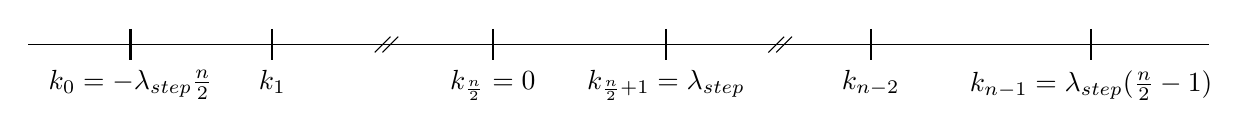
\begin{tikzpicture}
\foreach \x/\y in {
-6.2/ k_{0} = - \lambda_{step} \frac { n } { 2 } , 
-4.4/ k_{1},
0.6/ k_{ \frac{n}{2} + 1} = \lambda_{step} , 
-1.6/ k_{ \frac{n}{2}} = 0, 
3.2/ k_{n - 2}, 
6/ k_{n-1} =   \lambda_{step} (\frac { n } { 2 } - 1 )      }
 \draw[thick] (\x,0.2) -- (\x,-0.2) node[below]{$\y$};
\draw[thin] (-3,-0.10)--(-2.8 ,0.10);
\draw[thin] (-3.1,-0.10)--(-2.9 ,0.10);
\draw[thin] (1.9,-0.10)--(2.1 ,0.10);
\draw[thin] (2,-0.10)--(2.2 ,0.10);
\draw[thin] (-7.5,0)--(7.5 ,0);
\end{tikzpicture}
\end{figure}


parallelly, the frequencies where we evaluate the characteristic function are defined with another grid. Increasing the number of frequency points increases the precision of each price. We use a regular frequency-grid, with step $\eta_{step}$ yielding: $ \xi_j =j \cdot  \eta_{step}$, for $j \in \{ 0, \cdots, n-1 \} $. Now we can approximate the call price:


\begin{align}
C_T(k_u) &= \frac{ e^{- \alpha k_u }} {  \pi } \int_0^{\infty} e^{-i \xi k_u } \psi( \xi ) d \xi  \nonumber \\
& \approx \frac{ e^{- \alpha k_u }} {  \pi } \int_0^{ n \eta } e^{-i \xi k_u } \psi( \xi ) d \xi   \label{eq:truncation} \\
&\approx \frac{ e^{- \alpha k_u }} {  \pi } \sum_{j=0}^{n-1} 
a_j \exp \left ( - i k_u \xi_j \right )  \psi(\xi_j)   \label{eq:discrete} \\
& =  \frac{ e^{- \alpha k_u }} {  \pi } \sum_{j=0}^{n-1} 
a_j \exp \left ( 
i \cdot ( \lambda \frac n 2 - \lambda u ) \cdot \eta j 
\right )  \psi(\xi_j) 
\label{eq:final_form_pricing}
\end{align}

where the $a_j$ are the weights in the quadrature. With the composite Simpson's rule:

$$
a_j = \left\{
    \begin{array}{lll}
        \frac{ \eta_{step} } 3 & \mbox{if } j \in \{0,n-1 \}  \\
        4 \frac{  \eta_{step} } 3 & \mbox{elif } j \equiv 1 \;(\bmod\; 2) \\
        2 \frac{ \eta_{step} } 3 & \mbox{elif } j \equiv 0 \;(\bmod\; 2) \\
    \end{array}
\right.
$$

The last step, in order to apply the FFT algorithm, we apply a condition on the product $ \eta \lambda $, making the identification between (\ref{eq:FFT_form}) and (\ref{eq:final_form_pricing}) possible. This fixes: $ \lambda \eta = \frac {2 \pi } n $. Then, the final scheme looks like:

\begin{theoreme}{Pricing with the FFT and a closed form formula }
\begin{equation}
\label{eq:final_form_pricing_final}
C_T(k_u) = \frac{ e^{- \alpha k_u }} {  \pi } \sum_{j=0}^{n-1} 
a_j \exp \left ( 
- i \cdot \frac{2 \pi} {n} \cdot  u  \cdot   j 
\right ) 
e^{ i \pi  j }
\psi(\xi_j) 
\end{equation}
\end{theoreme}

A quick word about the introduced errors. The first error introduced in (\ref{eq:truncation}) is called a truncation error. It comes from the fact that the effective upper limit for the integration became, by truncation, $[0, n \eta ]$. Additionally, the integral is sampled in (\ref{eq:discrete}) for quadrature and results a sampling error. Intuitively, I would say that this error should be nicely bounded because we used the Simpson's method whose error is in $o( \frac 1 {n^4})$. However, we also saw that the function is highly oscillatory near $0$, then the bound upon the error might not be accurate. A more rigorous discussion of the error can be found in \cite{roger_lee}.





\subsection{Results}


The results are presented in the following figures: fig. \ref{fig:fft}.

The graph only shows prices near ATM. What happens is that one observes explosions for prices out of the money, due to the errors previously mentioned. Nevertheless, increasing the precision near the money comes with having prices out of the money, so zooming is a must. One notices that the prices are slightly scaled, but the shape corresponds. In order to check if the shape corresponds, I computed the ratio between the price given by the FFT and the price given by the close form formula. I plotted the ratios in fig. \ref{fig:fft_ratio}. It is clear that the ratio is not constant, however, for prices OTM and ATM, where also the price is not closed to zero, the ratio remains relatively constant ($[1.35,2]$), or at least, constant in a small neighbourhood. The ratio explodes in particular to prices far in the money, where the pricing is close to zero everywhere. It looks exponential for prices ITM.

Then, one can say the pricing is accurate, even though it has to be rescaled.


\begin{figure}
\centering
\includegraphics[width = 0.7 \textwidth]{../addition_part/images/integration_fft/fft.png}
\caption{Results of pricing with FFT.}
\label{fig:fft}
\end{figure}


\begin{figure}
\centering
\includegraphics[width = 0.7 \textwidth]{../addition_part/images/integration_fft/fft_ratio.png}
\caption{Verification of the pricing by FFT.}
\label{fig:fft_ratio}
\end{figure}





















\section{Implied Volatility}
\subsection{Definition}

\begin{definition}[Implied Volatility]

The implied volatility is a metric that captures the market's view of the likelihood of changes in a given security's price. 

It is deeply connected to the B$\&$S formula. 

Still in a philosophical way, the implied volatility is the volatility of the model if it was computed under the Black and Scholes model. As a result, estimating the IV allows to estimate how volatile a model is in comparison to a standard model. Then, if the former is riskier (resp. less), the premium for options should be higher (resp. lower). 

Mathematically, the B$\&$S formula can be inverted (cf. theorem \ref{thrm:BSformula} and appendix \ref{anx:invert_BS}). The implied volatility $ \sigma_{IV} $ is defined as the unique positive solution of:
\begin{equation}
\label{eq:IVunique}
C_{BS} ( S_0, K, T, \sigma_{IV} ) = C ( S_0, K, T )
\end{equation}

Then, IV helps us understand how the market estimates the volatility of a stock.

\end{definition}


One can see in fig. \ref{fig:BSvolatilitymaxcase} an example of the prices of the Heston model stuck between the two extreme cases of the Black and Scholes model (which corresponds to the extreme cases where the volatility has been taken to extremely high and low variance). Then, finding the $\sigma_{IV}$ that solves the equation is reduced to a root-finding problem.

One way to find the root is by using numerical efficient algorithms. The first one used is the bissect algorithm. Also, later, we test the efficiency of the Newton-Raphson algorithm.
\subsection{Implied Volatility for B$\&$S}
\begin{figure}
\centering
\subfloat{{
\includegraphics[width = 0.6 \textwidth]{../addition_part/images/BS/BSIV2.png}
}}\\
\subfloat{{
\includegraphics[width = 0.6 \textwidth]{../addition_part/images/BS/BSIV1.png}
}}\\
\subfloat{{
\includegraphics[width = 0.6 \textwidth]{../addition_part/images/BS/BSIV3.png}
}}\\
\caption{IV for B$\&$S in the case (parameters of B$\&$S: $r = 0, X_0 = 1$) of $\sigma = 0.03, 0.1, 0.3$.}
\label{BSIVflat}
\end{figure}

As one can expect from the definition, the IV for B$\&$S model should be flat. It is indeed flat to the extent of numerical errors, especially for strike prices far from ATM (cf. fig. \ref{BSIVflat}). Usually, the interesting strike prices are around $0$ on a range of 10$\%$. In other words, the flatness of the curve for the Black and Scholes model is verified. Also, one notices that the higher the variance, the less is the implied volatility influenced by large far ATM strike prices. This is explained by the fact that a greater volatility allows more flexibility for the convergence of the iterative algorithms. One can read section  \ref{diff_vega} for more details.

\subsection{Implied Volatility for Empirical pricing}
\label{section:IVempirical}
Fig. \ref{fig:IVempirical} shows the implied volatility of the pricing estimator. We use the same parameters as before (table \ref{table:parameters_for_closed_form}).

\begin{figure}
\centering
\includegraphics[width = 0.7 \textwidth]{../addition_part/images/integration_fft/IVempirical.png}
\caption{Implied Volatility of the empirical pricing for 5000 simulations. Closed form in red, empirical in purple. First set of parameters, from table \ref{table:parameters_for_closed_form}. }
\label{fig:IVempirical}
\end{figure}

The IV is pretty similar to the closed form one, which are respectively represented by the purple line and red dotted line. One can see that the IV gets to $0$ for log strikes prices higher than $1.8$. This is due to numerical errors. Also, one observes that the shape of the empirical IV gets further from the closed form's one as strike prices get more extreme. This is due to the fact that the estimator hasn't fully converged yet. So one can say that the empirical pricing is a good estimator of the price. Nevertheless, its precision decreases as one gets further from ATM prices.

Now, we change the parameters, and we plot again the empirical implied volatility. It is visible on fig. \ref{fig:IVempirical2}. We observe the same good behaviour of the estimator, confirming that the natural empirical estimator works correctly to estimate the price.

\begin{figure}
\centering
\includegraphics[width = 0.7 \textwidth]{../addition_part/images/integration_fft/IVempirical2.png}
\caption{Implied Volatility of the empirical pricing for 5000 simulations. Closed form in red, empirical in purple. Second set of parameters, from table \ref{table:parameters_for_closed_form}. }
\label{fig:IVempirical2}
\end{figure}

Finally, we want to see the impact of the number of random paths generated on the convergence of the estimator. One way to do it would be to compute the MSE of the estimator in order to check the consistency\footnote{Consistency follows from MSE convergence, cf. \cite{panaretos}.}. In order to not delve into too much details, we do a simple heuristic comparison.

With fig. \ref{fig:IVempirical_evol}, we plot the convergence of the estimator, in implied volatility scale, with respect to the number of random paths generated. We observe that more simulations increase the precision: the highest simulated number, represented by the purple shape, is closer to the dotted line, the latter corresponding to the true implied volatility. However, we see that when one goes further from ATM, the shape diverges. In fact, on the right (far ITM), the IV is constantly zero; on the left (far OTM), the IV is not computable anymore as the values are not invertible anymore.

An interesting thing to notice is that even though the prices are indeed all very close to the true price (left graph), the IV shapes are all different. Hence, the IV is a better indicator of convergence of the empirical estimator. However, it is also very sensible as one can see in fig. \ref{fig:IVempirical_evol2}. In the second graph, we plotted the same estimator, under the same parameters but for a number of simulations much higher. Now we observe that the estimator with the most simulations (60000 paths generated) is very far from the true IV. My rational for this phenomenon is that the estimator converged to the true price, modulo a numerical error, that stacks up as the number of simulations increases.

\begin{figure}
\centering
\includegraphics[width = 0.95 \textwidth]{../addition_part/images/integration_fft/low_IV_empirical.png}
\caption{Evolution of the empirical implied volatility for small amount of simulations. True IV in black. Parameters same as for \ref{fig:IVempirical_evol2}.}
\label{fig:IVempirical_evol}
\end{figure}


\begin{figure}
\centering
\includegraphics[width = 0.95 \textwidth]{../addition_part/images/integration_fft/high_IV_empirical.png}
\caption{Evolution of the empirical implied volatility for large number of simulations. True IV in black. Parameters of the simulation at the bottom of the image.}
\label{fig:IVempirical_evol2}
\end{figure}



\subsection{Computation}
The computation is given by that function, and fig. \ref{fig:iv_bissect} shows the result for a change of the vol of vol under the Heston model. We will shortly compare that graph to the one obtained from another method of root-finding.

\begin{verbatim}
def implied_volatility_empirical_heston(S, k, s0, T, R):
    ## s0 starting point of the S's,
    ## S realisation of the S_T
    my_price = empirical_price_option(S, k, T, R)

    def smile_min(vol, *args):
        k, s0, T, r, price = args
        return price - BlackScholes(True, s0, k, T, r, 0., vol)

    vMin = 0.000001
    vMax = 10.
    # in order to find the implied volatility, one has to 
    # find the value at which smile_min crosses zero. 
    return scipy.optimize.bisect(smile_min, vMin, vMax, 
    args=(k, s0, T, R, my_price), xtol=1e-20, rtol=1e-15,
    full_output=False, disp=True)
\end{verbatim}


\begin{figure}
\centering
   \includegraphics[width = 0.75 \textwidth]{../addition_part/images/integration_fft/Heston_IV.png}
   \caption{Implied volatility computed with bissect method.}
   \label{fig:iv_bissect}
\end{figure}











\subsection{Newton Raphson}
Another way to solve the implied volatility equation  (\ref{eq:IVunique}) is the Newton-Raphson. It is an efficient iterative algorithm to find the roots of a function, while using its derivative.

For more details about theory and convergence, I redirect anyone to the lecture notes of Albina Danilova: "Optimization with Applications in Portfolio Choice" (LSE). The main idea in Newton-Raphson algorithm lays upon the following equation:

$$ \sigma^{ \text{imp} }_{k+1} = \sigma^{ \text{imp} }_{k} - \frac{f\sigma^{ \text{imp} }_{k})}{  f'(\sigma^{ \text{imp} }_{k})} $$

or written equivalently, we are searching for the solution to the equation: 

$$ f(\sigma^{ \text{imp} }_{k}) + f'(\sigma^{ \text{imp} }_{k}) \cdot (\sigma^{ \text{imp} }_{k+1} -\sigma^{ \text{imp} }_{k} ) = 0 $$
Starting with an initial guess, the approximate solutions iteratively improve until a certain criterion is satisfied. The function $f$ and its derivative are given by the following. The latter is also referred to as "Vega". The computation of those formulas can be found in \ref{anx:invert_BS}.

\begin{align*}
f(x) &= C_{BS} - C_{Heston} \\
f'(x) &= \text{ VEGA } (C_{BS}) = S_0 N'(d_+)\sqrt{T}
\end{align*}



\begin{figure}
\centering
   \includegraphics[width = 0.75 \textwidth]{../addition_part/images/integration_fft/Heston_NEWTON_IV.png}
   \caption{Implied volatility computed with Newton Raphson method.}
   \label{fig:iv_newton}
\end{figure}

\begin{figure}
\centering
   \includegraphics[width = 0.75 \textwidth]{../addition_part/images/integration_fft/Implied_vol_heston_recommandation.png}
   \caption{Optimal $\sigma$ according to Brenner and Subrahmanyan in \cite{Brenner}.}
   \label{fig:brenner}
\end{figure}


A recommendation from \cite{Brenner} about the starting point in Newton-Raphson algorithm applied to the implied volatility is:
$$
   \sigma \approx \sqrt{\cfrac{2\pi}{T}} . \cfrac{C}{S}
$$

where $C$ is the price of the option with respect to the BS model, and $S$ is the spot price. 

It seemed to be a good starting point for options near the money. 
However, it didn't seem to be very conclusive far from ATM. In order to understand why, I plotted the previous equation as a function of the strike price. One can observe that this first guess reduces to zero extremely quickly (cf. fig. \ref{fig:brenner}). It makes this first guess not useful for values far from ATM. Also, under three different $\sigma$ for the model, the shapes of the guess were all relatively very close.

One can see the results of the searching algorithm used for computing the implied volatility in fig. \ref{fig:iv_newton}. It yields the same results (cf. fig. \ref{fig:iv_bissect}) and it seems that using Newton-Raphson takes as much time as to use the implemented method bisect. This must come from the fact that my function is not optimized. The code for Newton-Raphson is on appendix \ref{appendix_code:newton}.

\subsection{Difficulties}
\label{diff_vega}

The principal concern while using root finding algorithms is the failure of convergence. Bissect as well as Newton-Raphson method may fail to converge. Especially, when Vega is extremely small, making the function flat and leading to the stall of the convergence. One notices that the inversion giving the solution is a map from an unbounded interval to a finite one ( $\sigma \in [0, + \infty[ \to [0, S_0 - K e^{-rT} ]$ ). As a result, certain $\sigma-$regions are totally flat and Vega is really close to zero. This happens when the option is either far ITM or OTM. This is visible on fig. \ref{fig:vegabs}.

\subsection{Interpretation}

The typically observed implied volatility shapes in the market, for instance smile or skew, can be obtained by varying the parameters. 

Fig. \ref{fig:diff_sets_param} shows how parameters influence the shape of the implied volatility. The dotted lines have greater $\sigma$, the purple lines are references, the cyan lines have higher $\phi$ and the red ones opposed $\rho$. 

Then, we observe that $\sigma$ is proportional to a sharper curve (the kurtosis), $\phi$ shifts the implied volatility higher and $\rho$ shifts the IV in the more extreme moneyness direction (asymmetry).

\begin{figure}
\centering
   \includegraphics[width = 0.9 \textwidth]{../addition_part/images/integration_fft/comparaison_IV.png}
   \caption{Implied volatility for Heston with different parameters in order to observe their influence.}
   \label{fig:diff_sets_param}
\end{figure}






\section{Option Pricing using a Neural Network}
As personal work, I tried to price options using an artificial neural network (ANN). The target is the well-known B-S model.


\subsection{Data-set}

I generated a data-set randomly with this scheme (cf. table: \ref{table:data_ANN}). The number of data points is $10$e$6$. Usually people have access to huge data-set on financial markets so having a big data-set is not a farfetched hypothesis.


\begin{table}
\begin{tabular}{  | m{2.5cm} | m{4 cm} | m{4 cm}| m{4 cm}   } 
\hline
parameter & $S_0$ &  K & T   \\ 
\hline
\hline
values &$[5,80]$ & $[50,150]$\% & $[0.2,3]$  \\
\hline
method & randint$(500,8000)/100$ & randint$(50,150)/100$ & randint$(20,300$) $/ 100 $ \\
\hline
\end{tabular}
\end{table}



\begin{table}
\begin{tabular}{  m{4.5 cm} |m{4.5 cm} |m{4.5 cm} |  } 
\hline
 r & $\sigma $ & option type \\ 
\hline
\hline
 $[0,0.2]$ & $[0,0.8]$ & [call, put] \\
\hline
 randint$(1,2000) / 10000$ & randint$(1, 800)/100$  & choice(['Call','Put']) \\
\hline
\end{tabular}

\caption{Parameters for the training data-set}
\label{table:data_ANN}
\end{table}




Here, randint corresponds to a uniform distribution taken over the integers in the set. Choice is a uniform distribution over a discrete set.




The parameters correspond to the one in the B$\&$S formula.

In other words, $S_0$ is the original price of the underlying asset, $K$ is the strike price, $T$ is the time to maturity (in years), $r$ is the risk-free interest rate, $\sigma$ is the volatility of the asset.



\subsection{Architecture}

Then, I trained a neural network with the following characteristics  (cf. table \ref{table:architecture_ANN}, third column). The loss is computed with the mean square error, which seems to be fairly commonly used for continuous regressions. 

\begin{table}
\begin{center}
\begin{tabular}{   m{4.5 cm} | m{4.5 cm} | m{4.5 cm}   } 
\hline
 Parameters & Recommendation & My choice \\ 
\hline
\hline
Hidden Layers & $4$ & 2 \\
\hline
Neurons & $400$ & 400 \\
\hline
Activation & ReLU & ReLU \\
\hline
Dropout &$ 0.0$ & 0.0 \\
\hline
Batch Normalization & No &  No\\
\hline
Optimizer &  Adams & Adams \\
\hline
Batch Size & $1024$ & 4096 \\
\hline
Learning Rate & ?? & 0.000003 \\
\hline
Number of epochs & ?? &  120 \\
\hline
\end{tabular}
\caption{Architecture of the ANN.}
\label{table:architecture_ANN}
\end{center}
\end{table}

My choice of parameters was driven by one paper (cf. \cite{neuralnetworks1}) where a rigorous exploration of the parameters has been done. In the paper, they recommended the following choice (cf. table \ref{table:architecture_ANN}, second column). I chose to put less layers as I wanted to lower the number of parameters, and I increased the batch size because in my data-set I have many different possible combination of parameters. I wanted the neural network to see a subsequent range of the possible inputs.







\subsection{Results of training and validation}

Finally, my validation set is reduced to a curve for the sake of being able to plot it and see the results (cf. table \ref{table:validation_ANN}). 


\begin{table}
\centering
\begin{tabular}{  | m{2.5cm} | m{1.3 cm} | m{2 cm}| m{1.5 cm} |  m{1.2 cm} | m{1.2 cm}| m{2.4 cm} |  } 
\hline
parameter & $S_0$ &  $K$ & $T$ & $r$ & $\sigma$ & option type   \\ 
\hline
values &$50$ & $[75,140] S_0 \% $ & $1$ & $0.1$ & $0.5$ & Call  \\
\hline
\end{tabular}
\caption{Parameters for the validation data-set}
\label{table:validation_ANN}
\end{table}









\begin{figure}
\centering
\includegraphics[width = 0.8 \textwidth]{../addition_part/images/NN/loss_function.jpg}
\caption{Loss functions during training}
\label{im:loss_function}

\end{figure}




\begin{figure}
\centering
\includegraphics[width = 12cm]{../addition_part/images/NN/MSE.jpg}
\caption{Histogram of the mean square error during training}
\label{im:MSE}
\end{figure}







\begin{figure}
\centering
\includegraphics[width = \textwidth]{../addition_part/images/NN/prediction.jpg}
\caption{Plot of the prediction in the validation set.}
\label{im:prediction}
\end{figure}





We observe that the loss function decreases smoothly to $0.423$. This is confirmed by the histogram of the MSE that shows most points have a MSE that is less than $0.5$ ($85\%$ less than $0.5$ and $95\%$ less than $1$). Also, the prediction from the neural network (the purple line) is really close to the true value. This shows that the neural network provided a good fit for a random line. However, in order to know if the main characteristics of the curve are preserved, one has to use the implied volatility and see the shape of the curve.

Also, it is worth noting that the loss for the validation and for the training set are almost equal. Most probably, it is due to the high number of points in the data-set, and the low number of "new cases" in the validation data-set.


\subsection{Implied Volatility}

Fig. \ref{fig:iv_nn} shows the resulting implied volatility. We were expecting a flat IV since we try to approximate the B$\&$S model. Here we see that IV is negatively biased but fairly flat: the extremal variation represents merely $6\%$. For options in the money (moneyness around 50), the approximation is good (flatness: $1\%$ of change, bias of $4\%$).

\begin{figure}
\centering
\includegraphics[width = 0.7 \textwidth]{../addition_part/images/NN/IV_NN.jpg}
\caption{Implied Volatility of the prediction from the ANN.}
\label{fig:iv_nn}
\end{figure}




\subsection{Difficulties}


I faced two major difficulties with that task, namely


\begin{itemize}
  \item K-folding for continuous data.
  \item scalling data while still presenting meaningful plots.
\end{itemize}


K-folding allows verification about over fitting. The data-set is cut into $K$ parts, one is taken as a validation set and $K-1$ as a training part. It allows to keep track of the loss function not only for the training part, that will always reduce as the number of epochs increases, but also to see how the ANN reacts to data it has never seen (the validation set). A characteristic one would expect from the validation and training sets is that they have the same distribution for the predictors. Stratified K-folding is a way to maintain a similar distribution over the $K$ parts. This is relatively easy to do for discrete predictors, but much harder for continuous data-sets. In particular, sklearn doesn't have a pre-built function doing that. So I created my own K-folding function for continuous data-set.

Another concern was identifiability. It is obvious that our data is not scaled. For instance, the strike price is way bigger than the risk-free interest rates. So scaling is a must in order to use the data-set. However, in order to have meaningful graphs, I kept the original data-set.

Also, what I first did was setting the price range of the assets to be quite small ( $[0.1, 5]$ ) in the same range as the other parameters. However, I faced one problem: the loss function converged too fast and was not able to give me meaningful results.
My guess is that if the targets are too small, then the gradient for optimizing the parameters in the neural network is not able to move enough and the parameters aren't optimized. Setting the targets to be big allows the gradient to have more freedom and come closer to the true prediction. This problem is purely numerical. 
The scale shouldn't impact the price at all, as one can prove that the only meaningful parameter is the percentage of difference between the spot price, and the strike price.